% Generated by figures/_scene.py (Scene.render_tikz) for 'Fig 1 teaser flow'; do not edit by hand, re-run the figure script.
% 6.875 x 2.5 in at 100 %; needs \usetikzlibrary{arrows.meta}; images in Figures/fig1/.
{%
\definecolor{c1A1A1A}{HTML}{1A1A1A}%
\definecolor{c2B2F3A}{HTML}{2B2F3A}%
\definecolor{c2F7D32}{HTML}{2F7D32}%
\definecolor{c3F5F8F}{HTML}{3F5F8F}%
\definecolor{c5B5F6B}{HTML}{5B5F6B}%
\definecolor{c5E4A96}{HTML}{5E4A96}%
\definecolor{c5F5F5F}{HTML}{5F5F5F}%
\definecolor{c809EC2}{HTML}{809EC2}%
\definecolor{c9A9AA6}{HTML}{9A9AA6}%
\definecolor{c9D8CC4}{HTML}{9D8CC4}%
\definecolor{cA07800}{HTML}{A07800}%
\definecolor{cA8456E}{HTML}{A8456E}%
\definecolor{cB4B4B4}{HTML}{B4B4B4}%
\definecolor{cC4C6D2}{HTML}{C4C6D2}%
\definecolor{cCFD0D8}{HTML}{CFD0D8}%
\definecolor{cD091A7}{HTML}{D091A7}%
\definecolor{cE0B020}{HTML}{E0B020}%
\definecolor{cE6ECF3}{HTML}{E6ECF3}%
\definecolor{cEAE7F2}{HTML}{EAE7F2}%
\definecolor{cFFFFFF}{HTML}{FFFFFF}%
\begin{tikzpicture}[x=1in, y=1in]%
\useasboundingbox (0,0) rectangle (6.8750,2.5000);
\draw[draw=cCFD0D8, line width=0.000pt, fill=cCFD0D8, rounded corners=0.0800in] (2.3350,0.1950) rectangle (3.5150,2.2450);
\draw[draw=c809EC2, line width=1.000pt, fill=cE6ECF3, dash pattern=on 3.00pt off 2.00pt, rounded corners=0.0500in] (0.2400,1.3000) rectangle (1.2200,2.2800);
\draw[draw=cE0B020, line width=0.800pt, fill=cFFFFFF, dash pattern=on 2.40pt off 1.60pt, rounded corners=0.0400in] (1.2700,1.8300) rectangle (1.7200,2.2800);
\draw[draw=cD091A7, line width=0.800pt, fill=cFFFFFF, dash pattern=on 2.40pt off 1.60pt, rounded corners=0.0400in] (1.2700,1.3000) rectangle (1.7200,1.7500);
\draw[draw=c9D8CC4, line width=1.000pt, fill=cEAE7F2, rounded corners=0.0600in] (3.8600,1.3000) rectangle (6.8350,2.2800);
\draw[draw=c809EC2, line width=1.000pt, fill=cE6ECF3, dash pattern=on 3.00pt off 2.00pt, rounded corners=0.0500in] (0.2400,0.2300) rectangle (1.2200,1.2100);
\draw[draw=cE0B020, line width=0.800pt, fill=cFFFFFF, dash pattern=on 2.40pt off 1.60pt, rounded corners=0.0400in] (1.2700,0.7600) rectangle (1.7200,1.2100);
\draw[draw=cD091A7, line width=0.800pt, fill=cFFFFFF, dash pattern=on 2.40pt off 1.60pt, rounded corners=0.0400in] (1.2700,0.2300) rectangle (1.7200,0.6800);
\draw[draw=c9D8CC4, line width=1.000pt, fill=cEAE7F2, rounded corners=0.0600in] (3.8600,0.2300) rectangle (6.8350,1.2100);
\node[anchor=south west, inner sep=0] at (2.3000,0.2300) {
\includegraphics[width=1.1800in, height=2.0500in]{Figures/fig1/model_band.png}};
\node[anchor=south west, inner sep=0] at (0.2700,1.3300) {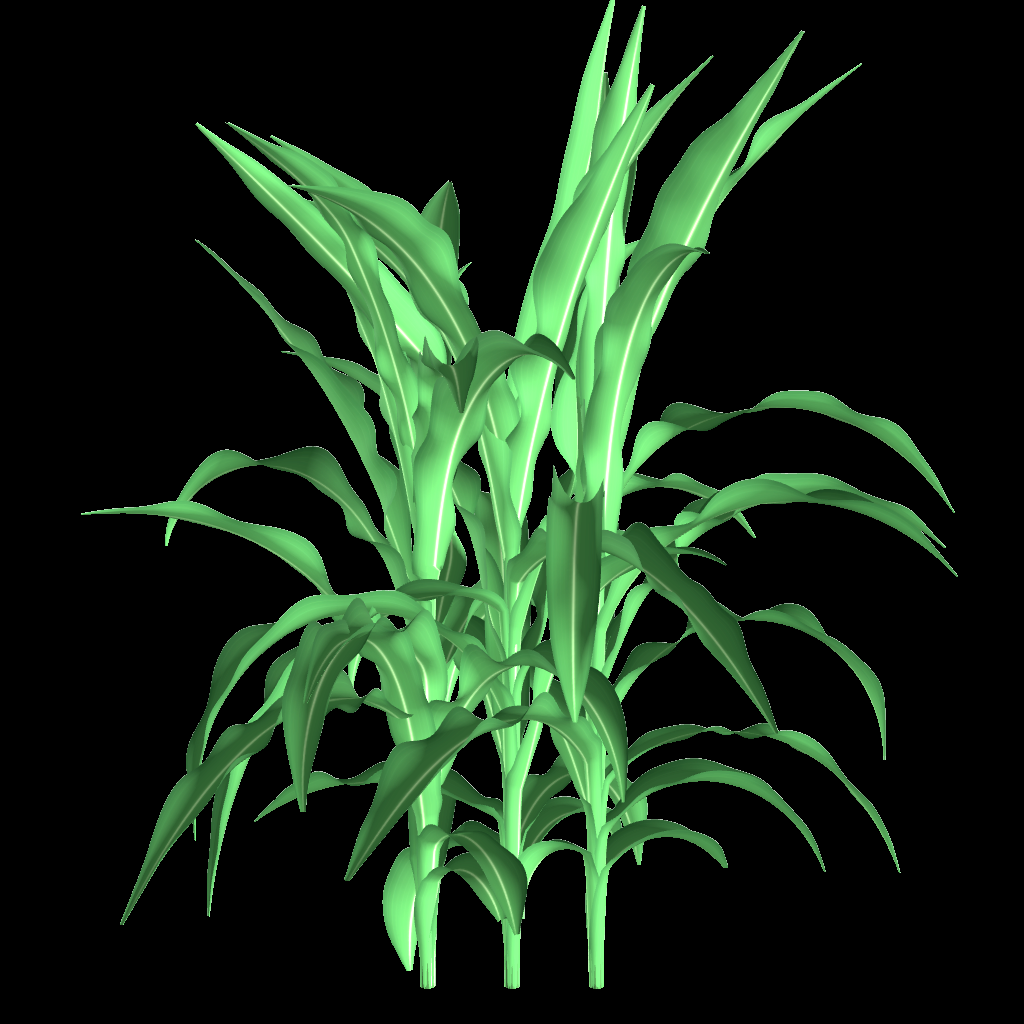
\includegraphics[width=0.9200in, height=0.9200in]{Figures/fig1/sorghum_row_photograph.png}};
\node[anchor=south west, inner sep=0] at (1.3000,1.8600) {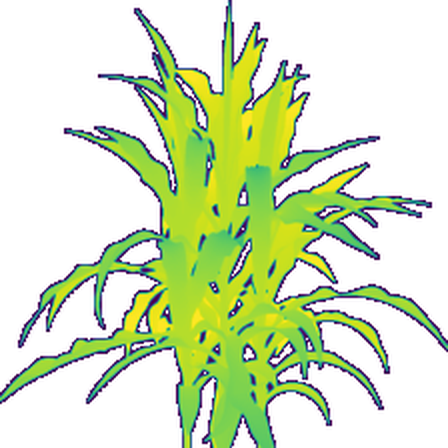
\includegraphics[width=0.3900in, height=0.3900in]{Figures/fig1/sorghum_depth.png}};
\node[anchor=south west, inner sep=0] at (1.3000,1.3300) {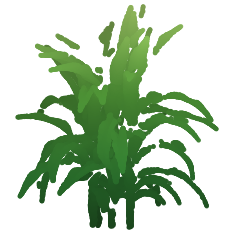
\includegraphics[width=0.3900in, height=0.3900in]{Figures/fig1/sorghum_pc.png}};
\node[anchor=south west, inner sep=0] at (3.8900,1.3300) {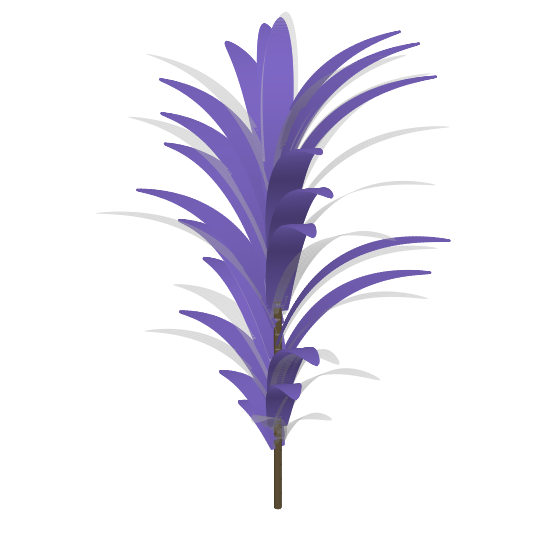
\includegraphics[width=0.9200in, height=0.9200in]{Figures/fig1/sorghum_procedural_plant.png}};
\node[anchor=south west, inner sep=0] at (0.2700,0.2600) {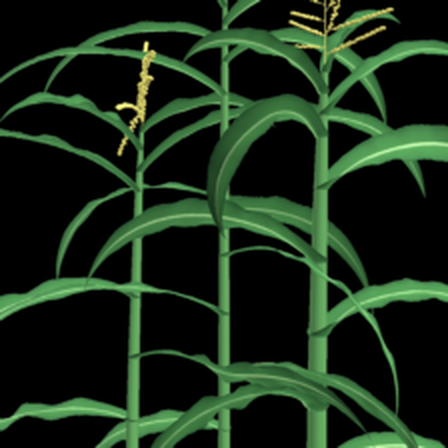
\includegraphics[width=0.9200in, height=0.9200in]{Figures/fig1/maize_row_photograph.png}};
\node[anchor=south west, inner sep=0] at (1.3000,0.7900) {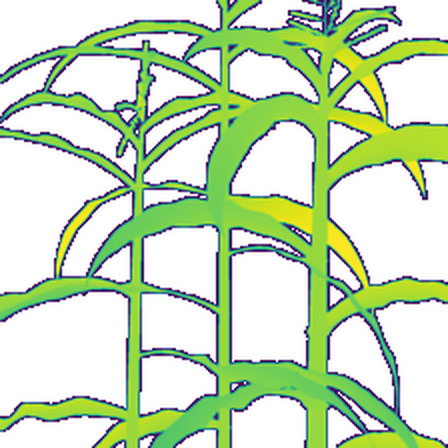
\includegraphics[width=0.3900in, height=0.3900in]{Figures/fig1/maize_depth.png}};
\node[anchor=south west, inner sep=0] at (1.3000,0.2600) {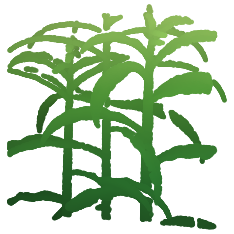
\includegraphics[width=0.3900in, height=0.3900in]{Figures/fig1/maize_pc.png}};
\node[anchor=south west, inner sep=0] at (3.8900,0.2600) {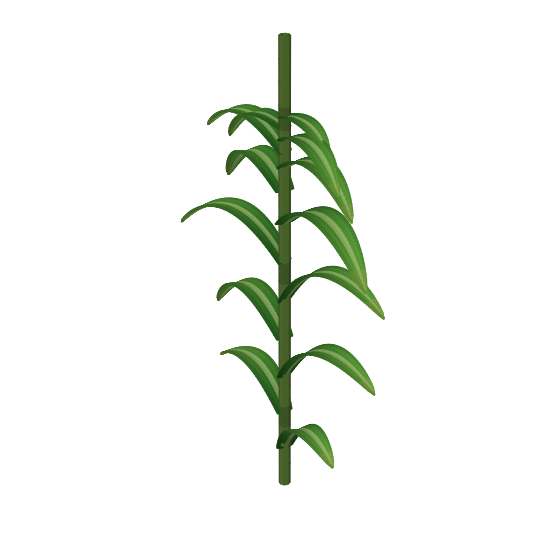
\includegraphics[width=0.9200in, height=0.9200in]{Figures/fig1/maize_procedural_plant.png}};
\draw[draw=c2B2F3A, line width=0.000pt, fill=c2B2F3A, rounded corners=0.1500in] (2.4000,1.8600) rectangle (3.3800,2.1600);
\draw[draw=cC4C6D2, line width=0.700pt, fill=cFFFFFF, rounded corners=0.0500in] (2.3700,1.2300) rectangle (3.4100,1.6100);
\draw[draw=cC4C6D2, line width=0.700pt, fill=cFFFFFF, rounded corners=0.0500in] (2.3700,0.7800) rectangle (3.4100,1.1600);
\draw[draw=cC4C6D2, line width=0.700pt, fill=cFFFFFF, rounded corners=0.0500in] (2.3700,0.3300) rectangle (3.4100,0.7100);
\draw[draw=c809EC2, line width=0.500pt, fill=c809EC2, rounded corners=0.0080in] (2.4300,1.4630) rectangle (2.4920,1.5250);
\draw[draw=c9A9AA6, line width=0.500pt, fill=cFFFFFF, rounded corners=0.0080in] (2.5040,1.4630) rectangle (2.5660,1.5250);
\draw[draw=cD091A7, line width=0.500pt, fill=cD091A7, rounded corners=0.0080in] (2.5780,1.4630) rectangle (2.6400,1.5250);
\draw[draw=c9A9AA6, line width=0.500pt, fill=cFFFFFF, rounded corners=0.0080in] (2.4300,1.3890) rectangle (2.4920,1.4510);
\draw[draw=c809EC2, line width=0.500pt, fill=c809EC2, rounded corners=0.0080in] (2.5040,1.3890) rectangle (2.5660,1.4510);
\draw[draw=c9A9AA6, line width=0.500pt, fill=cFFFFFF, rounded corners=0.0080in] (2.5780,1.3890) rectangle (2.6400,1.4510);
\draw[draw=c9A9AA6, line width=0.500pt, fill=cFFFFFF, rounded corners=0.0080in] (2.4300,1.3150) rectangle (2.4920,1.3770);
\draw[draw=c9D8CC4, line width=0.500pt, fill=c9D8CC4, rounded corners=0.0080in] (2.5040,1.3150) rectangle (2.5660,1.3770);
\draw[draw=c9A9AA6, line width=0.500pt, fill=cFFFFFF, rounded corners=0.0080in] (2.5780,1.3150) rectangle (2.6400,1.3770);
\node[anchor=south west, inner sep=0] at (2.4225,0.9075) {
\includegraphics[width=0.1250in, height=0.1250in]{Figures/fig1/snow.png}};
\node[anchor=south west, inner sep=0] at (2.5795,0.9075) {
\includegraphics[width=0.1250in, height=0.1250in]{Figures/fig1/fire.png}};
\draw[draw=c2B2F3A, line width=0.000pt, fill=c2B2F3A] (2.3700,1.5600) ellipse [x radius=0.0500, y radius=0.0500];
\draw[draw=c2B2F3A, line width=0.000pt, fill=c2B2F3A] (2.3700,1.1100) ellipse [x radius=0.0500, y radius=0.0500];
\draw[draw=c2B2F3A, line width=0.000pt, fill=c2B2F3A] (2.3700,0.6600) ellipse [x radius=0.0500, y radius=0.0500];
\draw[draw=c5B5F6B, line width=1.300pt, rounded corners=0.0800in] (2.3000,0.2300) rectangle (3.4800,2.2800);
\draw[draw=c2F7D32, line width=0.600pt, dash pattern=on 1.80pt off 1.20pt, rounded corners=0.0100in] (2.5070,0.4050) rectangle (2.5770,0.6400);
\draw[draw=cFFFFFF, line width=0.700pt, dash pattern=on 2.10pt off 1.40pt, rounded corners=0.0100in] (0.4233,1.3485) rectangle (0.9828,2.2500);
\draw[draw=cFFFFFF, line width=0.700pt, dash pattern=on 2.10pt off 1.40pt, rounded corners=0.0100in] (0.2700,0.2600) rectangle (1.1562,1.1800);
\node[anchor=west, inner sep=0, outer sep=0, align=left, text=c3F5F8F, font={\fontsize{8.50}{10.62}\selectfont\sffamily\bfseries}] at (0.2400,2.4000) {INPUT};
\node[anchor=west, inner sep=0, outer sep=0, align=left, text=c5F5F5F, font={\fontsize{8.50}{10.62}\selectfont\sffamily}] at (0.7400,2.4000) {any subset, from an occluded row};
\node[anchor=west, inner sep=0, outer sep=0, align=left, text=c5E4A96, font={\fontsize{8.50}{10.62}\selectfont\sffamily\bfseries}] at (3.8600,2.4000) {OUTPUT};
\node[anchor=west, inner sep=0, outer sep=0, align=left, text=c5F5F5F, font={\fontsize{8.50}{10.62}\selectfont\sffamily}] at (4.5800,2.4000) {procedural plant};
\node[anchor=center, inner sep=0, outer sep=0, align=center, text=cFFFFFF, font={\fontsize{11.00}{13.75}\selectfont\sffamily\bfseries}] at (2.8900,2.0100) {CropCode};
\node[anchor=center, inner sep=0, outer sep=0, align=center, text=c5F5F5F, font={\fontsize{7.50}{9.38}\selectfont\sffamily}] at (2.8900,1.7300) {one model, three stages};
\node[anchor=west, inner sep=0, outer sep=0, align=left, text=c1A1A1A, font={\fontsize{7.50}{7.88}\selectfont\sffamily}] at (2.7500,1.4200) {masked\\pretraining};
\node[anchor=center, inner sep=0, outer sep=0, align=center, text=cFFFFFF, font={\fontsize{6.50}{8.12}\selectfont\sffamily\bfseries}] at (2.3700,1.5600) {1};
\draw[draw=c5B5F6B, line width=1.000pt, -{Triangle[length=2.00pt,width=2.00pt]}] (2.5500,0.9700) -- (2.5850,0.9700);
\node[anchor=west, inner sep=0, outer sep=0, align=left, text=c1A1A1A, font={\fontsize{7.50}{7.88}\selectfont\sffamily}] at (2.7500,0.9700) {cross-modal\\distillation};
\node[anchor=center, inner sep=0, outer sep=0, align=center, text=cFFFFFF, font={\fontsize{6.50}{8.12}\selectfont\sffamily\bfseries}] at (2.3700,1.1100) {2};
\draw[draw=cB4B4B4, line width=1.000pt] (2.4650,0.4200) -- (2.4650,0.6200);
\draw[draw=cB4B4B4, line width=0.900pt] (2.4650,0.4750) .. controls (2.4868,0.4821) and (2.4982,0.4971) .. (2.4990,0.5200);
\draw[draw=cB4B4B4, line width=0.900pt] (2.4650,0.5150) .. controls (2.4432,0.5221) and (2.4318,0.5371) .. (2.4310,0.5600);
\draw[draw=cB4B4B4, line width=0.900pt] (2.4650,0.5550) .. controls (2.4868,0.5621) and (2.4982,0.5771) .. (2.4990,0.6000);
\draw[draw=c2F7D32, line width=1.000pt] (2.5420,0.4200) -- (2.5420,0.6200);
\draw[draw=c2F7D32, line width=0.900pt] (2.5420,0.4750) .. controls (2.5638,0.4821) and (2.5752,0.4971) .. (2.5760,0.5200);
\draw[draw=c2F7D32, line width=0.900pt] (2.5420,0.5150) .. controls (2.5202,0.5221) and (2.5088,0.5371) .. (2.5080,0.5600);
\draw[draw=c2F7D32, line width=0.900pt] (2.5420,0.5550) .. controls (2.5638,0.5621) and (2.5752,0.5771) .. (2.5760,0.6000);
\draw[draw=cB4B4B4, line width=1.000pt] (2.6190,0.4200) -- (2.6190,0.6200);
\draw[draw=cB4B4B4, line width=0.900pt] (2.6190,0.4750) .. controls (2.6408,0.4821) and (2.6522,0.4971) .. (2.6530,0.5200);
\draw[draw=cB4B4B4, line width=0.900pt] (2.6190,0.5150) .. controls (2.5972,0.5221) and (2.5858,0.5371) .. (2.5850,0.5600);
\draw[draw=cB4B4B4, line width=0.900pt] (2.6190,0.5550) .. controls (2.6408,0.5621) and (2.6522,0.5771) .. (2.6530,0.6000);
\node[anchor=west, inner sep=0, outer sep=0, align=left, text=c1A1A1A, font={\fontsize{7.50}{7.88}\selectfont\sffamily}] at (2.7500,0.5200) {row\\fine-tuning};
\node[anchor=center, inner sep=0, outer sep=0, align=center, text=cFFFFFF, font={\fontsize{6.50}{8.12}\selectfont\sffamily\bfseries}] at (2.3700,0.6600) {3};
\node[anchor=center, inner sep=0, outer sep=0, align=center, text=c1A1A1A, font={\fontsize{8.50}{10.62}\selectfont\sffamily\bfseries}, rotate=90] at (0.1000,1.7900) {Sorghum};
\node[anchor=south west, inner sep=0, outer sep=0, align=left, text=cFFFFFF, font={\fontsize{7.00}{8.75}\selectfont\sffamily}] at (0.3100,1.3800) {27 \% hidden};
\node[anchor=north west, inner sep=0, outer sep=0, align=left, text=cA07800, font={\fontsize{7.00}{8.75}\selectfont\sffamily}] at (1.7700,2.2600) {depth};
\node[anchor=south west, inner sep=0, outer sep=0, align=left, text=cA8456E, font={\fontsize{7.00}{8.75}\selectfont\sffamily}] at (1.7700,1.3200) {cloud};
\draw[draw=c809EC2, line width=1.800pt, -{Triangle[length=3.20pt,width=3.20pt]}] (1.2300,1.7900) -- (2.2800,1.7900);
\draw[draw=cE0B020, line width=1.800pt, -{Triangle[length=3.20pt,width=3.20pt]}] (1.7400,2.0550) .. controls (1.9092,1.9433) and (2.0892,1.9217) .. (2.2800,1.9900);
\draw[draw=cD091A7, line width=1.800pt, -{Triangle[length=3.20pt,width=3.20pt]}] (1.7400,1.5250) .. controls (1.9092,1.6367) and (2.0892,1.6583) .. (2.2800,1.5900);
\node[anchor=west, inner sep=0, outer sep=0, align=left, text=c5E4A96, font={\fontsize{8.50}{10.62}\selectfont\sffamily\bfseries}] at (4.9400,2.1000) {written by CropCode};
\node[anchor=west, inner sep=0, outer sep=0, align=left, text=c5F5F5F, font={\fontsize{8.50}{10.62}\selectfont\sffamily\bfseries}] at (6.3200,2.1000) {true};
\node[anchor=west, inner sep=0, outer sep=0, align=left, text=c5F5F5F, font={\fontsize{8.50}{10.62}\selectfont\sffamily}] at (4.9400,1.8600) {height};
\node[anchor=west, inner sep=0, outer sep=0, align=left, text=c5E4A96, font={\fontsize{8.50}{10.62}\selectfont\sffamily\bfseries}] at (5.7400,1.8600) {0.93 m};
\node[anchor=west, inner sep=0, outer sep=0, align=left, text=c5F5F5F, font={\fontsize{8.50}{10.62}\selectfont\sffamily}] at (6.3200,1.8600) {0.94 m};
\node[anchor=west, inner sep=0, outer sep=0, align=left, text=c5F5F5F, font={\fontsize{8.50}{10.62}\selectfont\sffamily}] at (4.9400,1.6700) {leaves};
\node[anchor=west, inner sep=0, outer sep=0, align=left, text=c5E4A96, font={\fontsize{8.50}{10.62}\selectfont\sffamily\bfseries}] at (5.7400,1.6700) {19};
\node[anchor=west, inner sep=0, outer sep=0, align=left, text=c5F5F5F, font={\fontsize{8.50}{10.62}\selectfont\sffamily}] at (6.3200,1.6700) {19};
\node[anchor=west, inner sep=0, outer sep=0, align=left, text=c5F5F5F, font={\fontsize{8.50}{10.62}\selectfont\sffamily}] at (4.9400,1.4800) {leaf length};
\node[anchor=west, inner sep=0, outer sep=0, align=left, text=c5E4A96, font={\fontsize{8.50}{10.62}\selectfont\sffamily\bfseries}] at (5.7400,1.4800) {0.74 m};
\node[anchor=west, inner sep=0, outer sep=0, align=left, text=c5F5F5F, font={\fontsize{8.50}{10.62}\selectfont\sffamily}] at (6.3200,1.4800) {0.76 m};
\draw[draw=c9D8CC4, line width=1.800pt, -{Triangle[length=3.20pt,width=3.20pt]}] (3.5000,1.7900) -- (3.8400,1.7900);
\node[anchor=center, inner sep=0, outer sep=0, align=center, text=c1A1A1A, font={\fontsize{8.50}{10.62}\selectfont\sffamily\bfseries}, rotate=90] at (0.1000,0.7200) {Maize};
\node[anchor=south west, inner sep=0, outer sep=0, align=left, text=cFFFFFF, font={\fontsize{7.00}{8.75}\selectfont\sffamily}] at (0.3100,0.3100) {22 \% hidden};
\node[anchor=north west, inner sep=0, outer sep=0, align=left, text=cA07800, font={\fontsize{7.00}{8.75}\selectfont\sffamily}] at (1.7700,1.1900) {depth};
\node[anchor=south west, inner sep=0, outer sep=0, align=left, text=cA8456E, font={\fontsize{7.00}{8.75}\selectfont\sffamily}] at (1.7700,0.2500) {cloud};
\draw[draw=c809EC2, line width=1.800pt, -{Triangle[length=3.20pt,width=3.20pt]}] (1.2300,0.7200) -- (2.2800,0.7200);
\draw[draw=cE0B020, line width=1.800pt, -{Triangle[length=3.20pt,width=3.20pt]}] (1.7400,0.9850) .. controls (1.9092,0.8733) and (2.0892,0.8517) .. (2.2800,0.9200);
\draw[draw=cD091A7, line width=1.800pt, -{Triangle[length=3.20pt,width=3.20pt]}] (1.7400,0.4550) .. controls (1.9092,0.5667) and (2.0892,0.5883) .. (2.2800,0.5200);
\node[anchor=west, inner sep=0, outer sep=0, align=left, text=c5E4A96, font={\fontsize{8.50}{10.62}\selectfont\sffamily\bfseries}] at (4.9400,1.0300) {written by CropCode};
\node[anchor=west, inner sep=0, outer sep=0, align=left, text=c5F5F5F, font={\fontsize{8.50}{10.62}\selectfont\sffamily\bfseries}] at (6.3200,1.0300) {true};
\node[anchor=west, inner sep=0, outer sep=0, align=left, text=c5F5F5F, font={\fontsize{8.50}{10.62}\selectfont\sffamily}] at (4.9400,0.7900) {height};
\node[anchor=west, inner sep=0, outer sep=0, align=left, text=c5E4A96, font={\fontsize{8.50}{10.62}\selectfont\sffamily\bfseries}] at (5.7400,0.7900) {1.07 m};
\node[anchor=west, inner sep=0, outer sep=0, align=left, text=c5F5F5F, font={\fontsize{8.50}{10.62}\selectfont\sffamily}] at (6.3200,0.7900) {1.06 m};
\node[anchor=west, inner sep=0, outer sep=0, align=left, text=c5F5F5F, font={\fontsize{8.50}{10.62}\selectfont\sffamily}] at (4.9400,0.6000) {leaves};
\node[anchor=west, inner sep=0, outer sep=0, align=left, text=c5E4A96, font={\fontsize{8.50}{10.62}\selectfont\sffamily\bfseries}] at (5.7400,0.6000) {13};
\node[anchor=west, inner sep=0, outer sep=0, align=left, text=c5F5F5F, font={\fontsize{8.50}{10.62}\selectfont\sffamily}] at (6.3200,0.6000) {13};
\node[anchor=west, inner sep=0, outer sep=0, align=left, text=c5F5F5F, font={\fontsize{8.50}{10.62}\selectfont\sffamily}] at (4.9400,0.4100) {leaf length};
\node[anchor=west, inner sep=0, outer sep=0, align=left, text=c5E4A96, font={\fontsize{8.50}{10.62}\selectfont\sffamily\bfseries}] at (5.7400,0.4100) {0.36 m};
\node[anchor=west, inner sep=0, outer sep=0, align=left, text=c5F5F5F, font={\fontsize{8.50}{10.62}\selectfont\sffamily}] at (6.3200,0.4100) {0.37 m};
\draw[draw=c9D8CC4, line width=1.800pt, -{Triangle[length=3.20pt,width=3.20pt]}] (3.5000,0.7200) -- (3.8400,0.7200);
\node[anchor=west, inner sep=0, outer sep=0, align=left, text=c5F5F5F, font={\fontsize{7.00}{8.75}\selectfont\sffamily}] at (0.2400,0.0700) {no mask or bounding box given  ·  here: all three streams (any subset is accepted)};
\node[anchor=east, inner sep=0, outer sep=0, align=right, text=c5E4A96, font={\fontsize{7.50}{9.38}\selectfont\sffamily}] at (6.8350,0.0700) {kilobytes  ·  editable  ·  re-renderable};
\end{tikzpicture}%
}%
